\documentclass[a4paper,11pt,onecolumn]{report}
\usepackage[T1]{fontenc} % Fontes T1
\usepackage[utf8]{inputenc} % Input UTF8
\usepackage[backend=biber, style=ieee]{biblatex} % para usar bibliografia
\usepackage{csquotes}
\usepackage[portuguese]{babel} %Usar língua inglesa
\usepackage{blindtext} % Gerar texto automáticamente
\usepackage[printonlyused]{acronym}
\usepackage{hyperref} % para autoref
\usepackage{graphicx}
\usepackage{minted}
\usepackage{indentfirst}
\usepackage{array}
\newcolumntype{L}[1]{>{\raggedright\let\newline\\\arraybackslash\hspace{0pt}}m{#1}}
\newcolumntype{C}[1]{>{\centering\let\newline\\\arraybackslash\hspace{0pt}}m{#1}}
\newcolumntype{R}[1]{>{\raggedleft\let\newline\\\arraybackslash\hspace{0pt}}m{#1}}


\bibliography{bibliografia}
\addbibresource{bibliografia.bib}


\begin{document}
%%
% Definições
%
\def\titulo{Temporizador de Reação}
\def\data{06/05/2015}
\def\autores{Pedro Martins, Pedro Santos}
\def\autorescontactos{pbmartins@ua.pt, pedroamaralsantos@ua.pt}
\def\versao{1}
\def\departamento{Departamento de Eletrónica Telecomunicações e Informática}
\def\empresa{Universidade de Aveiro}
\def\logotipo{ua.pdf}
%
%% CAPA %%
%
\begin{titlepage}

\begin{center}
%
\vspace*{50mm}
%
{\Huge \titulo}\\ 
%
\vspace{10mm}
%
{\Large \empresa}\\
%
\vspace{10mm}
%
{\LARGE \autores}\\ 
%
%
\vspace{30mm}
%
\begin{figure}[h]
\center
\includegraphics{\logotipo}
\end{figure}
%
\vspace{30mm}
\end{center}
%
\begin{flushright}
\versao
\end{flushright}
\end{titlepage}

%
%
%%  Página de Título %%
%
%
\title{%
{\Huge\textbf{\titulo}}\\
{\Large \departamento\\ \empresa}
}
%
\author{%
    \autores \\
    \autorescontactos
}
%
\date{\data}
%
\maketitle

%%%%%%%%%%%%%%%%%%%%%%%%%%%%%%%%%%%%%%%%%%%
% RESUMO
%
%
\pagenumbering{roman}

\tableofcontents


%%%%%%%%%%%%%%%%%%%%%%%%%%%%%%%
\clearpage
\pagenumbering{arabic}

%%%%%%%%%%%%%%%%%%%%%%%%%%%%%%%%
\chapter{Introdução}
\label{chap.introducao}

Para avaliação da componente prática da disciplina de Laboratórios de Sistemas Digitais, foi-nos proposto a criação de um mini-projeto, no qual teríamos de criar uma arquitetura e os seus variados blocos em \ac{vhdl}, a qual seria utilizada para programar uma \ac{fpga}, a Terasic DE2-115. Foi determinado pelo grupo que seria implementado um simples temporizador de reação, no qual seria utilizado botões e \textit{switches} da \ac{fpga}, assim como um comando infravermelhos, de maneira a que seja possível jogar em ambas as plataformas. Para a construção do projeto, foram utilizadas máquinas de estados, assim como blocos de lógica simples e ainda as \textit{blackboxes} relativas às interfaces de infravermelhos e áudio, disponibilizadas pelos docentes da disciplina.

\chapter{Análise}
\label{chap.analise}
O mini-projeto em análise consiste na implementação de um temporizador de reação. A ideia pode traduzir-se como, depois de aceso um LED, medir o tempo que o utilizador demora a carregar num botão pré-definido, registando o tempo decorrido entre ambos. 

Como foi implementado um descodificador de infravermelhos, pode utilizar-se tanto o comando (desde que este envie informação no formato NEC), como os botões e \textit{switches} da \ac{fpga}. 

Assim sendo, existe um botão (\texttt{KEY(0)}) na \ac{fpga} e outro no comando (botão de Play) para iniciar o jogo e que também terá como função parar o cronómetro que contabilizará o tempo de reação assim que o LED é ligado.

Existirá também um botão que servirá para fazer \textit{Reset} ao sistema em qualquer ponto do seu funcionamento ( \texttt{KEY(0)} na \ac{fpga} e Return no comando), e um botão para parametrizar o tempo de espera antes de aparecer o LED verde, que simboliza o início da contagem do tempo de reação. Caso esteja ativo o \texttt{SW(0)} da \ac{fpga}, esse tempo será definido como 5 segundos, caso contrário será um valor aleatório. No entanto, existe um funcionalidade exclusiva ao comando de infravermelhos. Para além de se poder parametrizar o valor de espera, usando a tecla QUALQUERCOISA, também é possível escolher esse valor, desde que esteja no intervalo entre 1 e 9 segundos (utilizando para o efeito os botões de 1 a 9 disponíveis no comando).

Assim que o utilizador carrega no botão de iniciar o jogo, é gerado um número aleatório entre 5 e 60 (e validado), que será o tempo, em segundos, que demorará o LED a acender desde que se iniciou o jogo. De seguida, é utilizado um "semáforo de partida", onde a cada segundo, 3 LED vermelhos se apagam e onde é emitido um som, até que se inicia a contagem do tempo até o LED indicador se acender.

Se o utilizador carregar no botão de jogar antes de o LED acender, é impresso nos ecrãs hexadecimais uma mensagem de erro. Caso o utilizador apenas clique no botão depois de aceso, é imprimido nos ecrãs hexadecimais o tempo percorrido desde que o LED acendeu até o utilizador carregar no botão. A \ac{fpga} manter-se-á neste estado até que se reinicie o jogo, isto é, clicar no botão de \textit{Reset}, onde todos os painéis hexadecimais e todos os LED serão apagados.

\section{Arquitetura}

\section{Arquitetura}
A figura \autoref{figblocos} apresenta uma arquitetura do sistema em geral.

%figura 1%
\begin{figure}[h]
\centerline{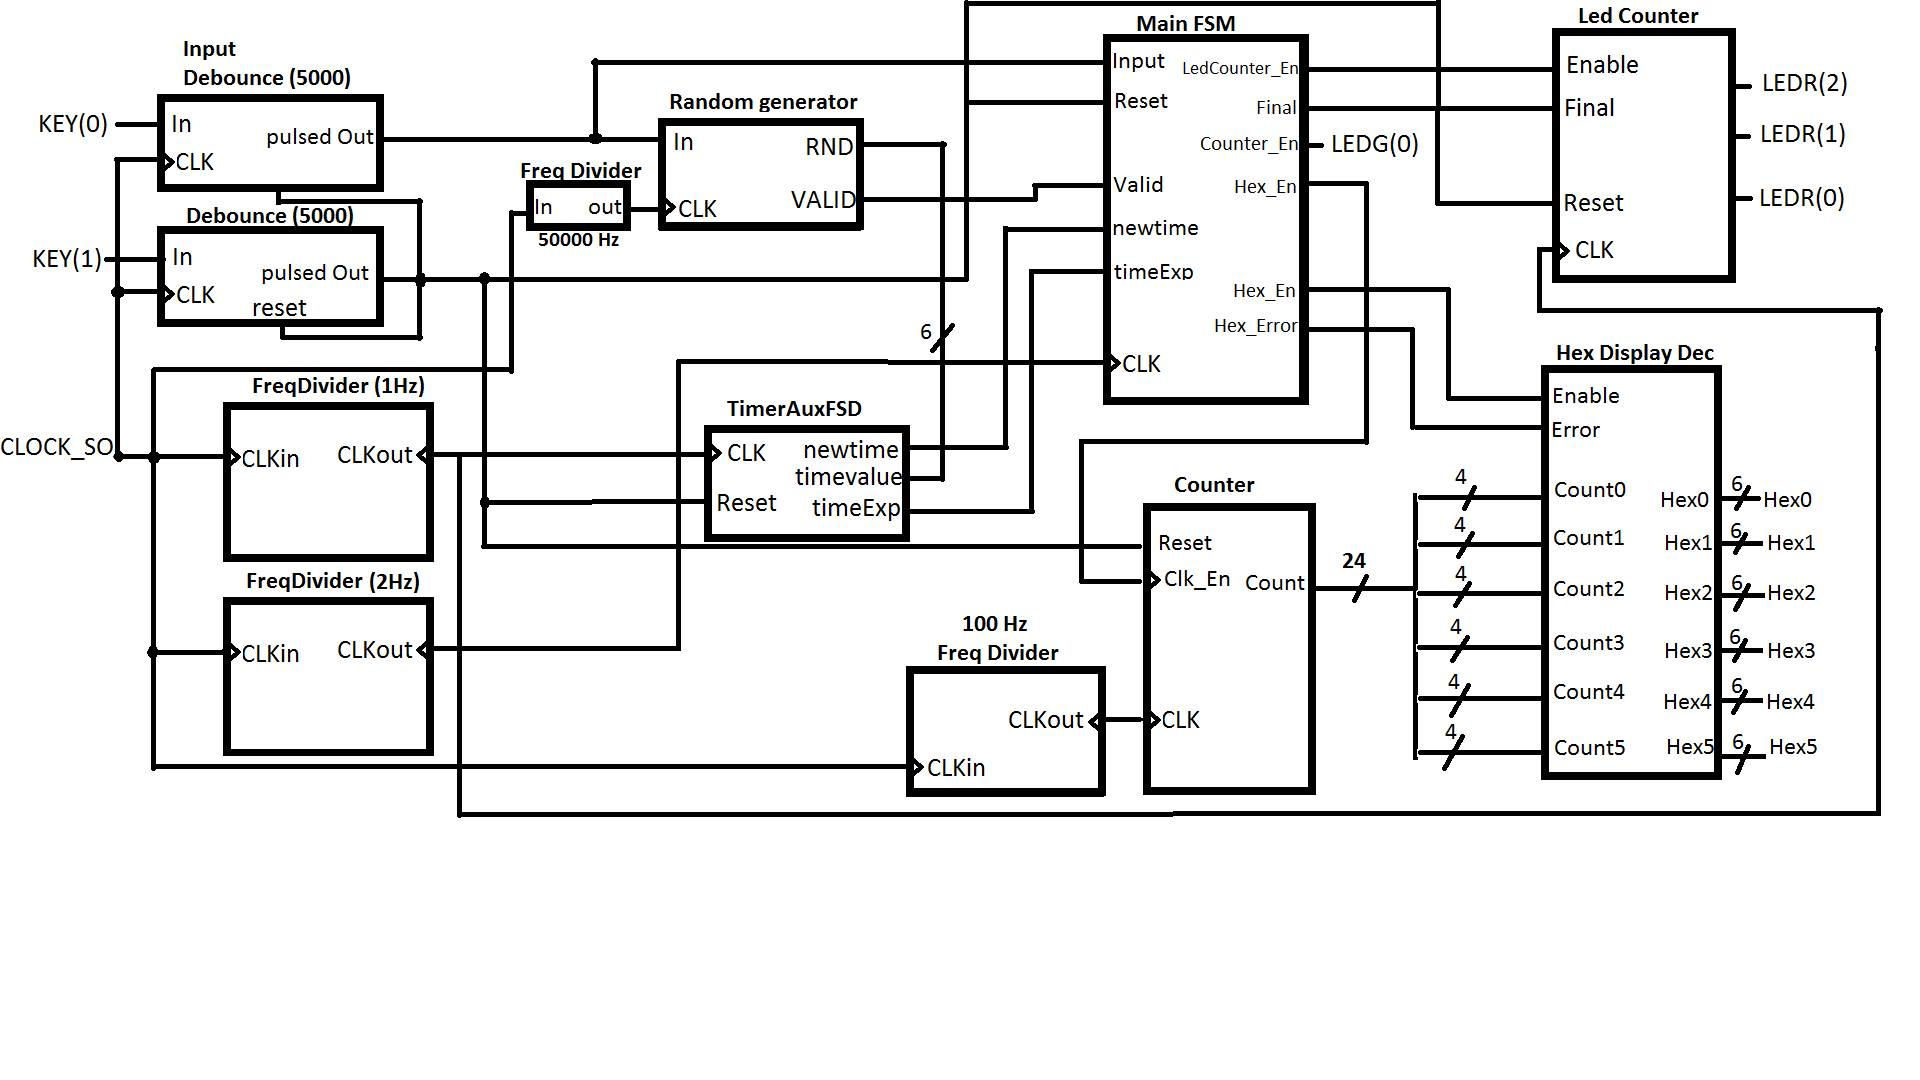
\includegraphics[scale=0.25]{Images/BlockDiagram}}
\caption{Arquitetura do temporizador de reação.}
\label{figblocos}
\end{figure}


\section{Implementação}

Este projeto foi construído tendo como base do seu funcionamento blocos lógicos simples, assim como máquinas de estados.

Primeiramente, é importante referir que os sinais proveniente dos botões \texttt{KEY} da \ac{fpga}, foram todos passados por um \textit{Debouncer} (bloco baseado num com a mesma função desenvolvido nas aulas), de modo a que não haja oscilações na altura do clique e seja enviado apenas um impulso.

Por outro lado, o descodificador de infravermelhos também foi baseado no fornecido pelos docentes da disciplina. Foram modificados vários aspetos, nomeadamente as funções associadas a cada botão e um analisador de impulsos, para que o sinal não seja sempre contínuo (por exemplo, para o caso em que se clica no botão Play: se o sinal fosse contínuo, quando clicássemos nesse botão, ele ia estar sempre ativo e ia, mesmo antes de aparecer o LED indicador, ele dar a mensagem de error de clicar no botão de jogar antes de o LED acender).

\subsection{\textit{Main FSM}}

O "cérebro" de todo o projeto é a máquina de estados \textit{Main FSM}. É ela que gere as ativações de todos os blocos e máquinas de estados auxiliares, consoante as entradas do dispositivo (botões da \ac{fpga} e comando de infravermelhos), assim como consoante os sinais provenientes dos restantes blocos.

%figura 5%
\begin{figure}[h]
\centerline{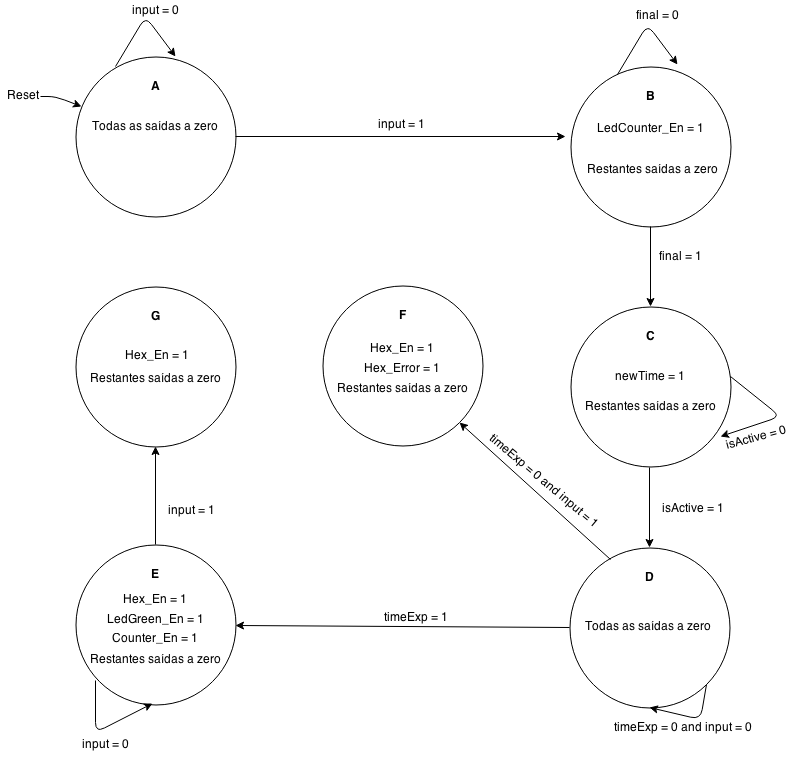
\includegraphics[scale=0.4]{Images/MainFSMDiagram}}
\caption{Diagrama de estados da \textit{Main FSM}.}
\label{figmainfsm}
\end{figure}

\subsection{\textit{LEDCounter FSM}}

Assim que é iniciado o jogo, é dado um "sinal de partida", gerado pela \textit{LEDCounter FSM}. Esta máquina de estados, que tem um relógio de frequência 2Hz (0.5 segundos - gerado pelo bloco \textit{FreqDivider}), recebe um sinal que a ativa, ligando três LEDs vermelhos, e, a cada dois tiques de relógio, vai desligando-os um a um. Para além disso, a cada tique, envia um sinal de \texttt{enable}, que ativa e desativa o bloco \textit{Audio\_Core}, responsável pela geração de um som e comunicação com a \textit{blackbox} da interface áudio, que resultará na emissão de um som alternadamente ligado (nos dois primeiros LEDs) e continuamente ligado (no último LED), até que todos sejam desligados.

O bloco \textit{Audio\_Core} é baseado no bloco \textit{AudioDemo} fornecido pelos professores como exemplo de interação com a interface áudio do kit Terasic DE2-115. Apenas foi modificado canal direito de saída, para este emitir o mesmo som que o da esquerda simultaneamente.

Ou seja, esta máquina funciona como um "semáforo de partida" e que, quando desligados todos os LEDs, inicia a contagem do tempo até que o LED verde (indicador) se acenda.

No entanto, se o \texttt{SW(1)} na \ac{fpga} estiver ativo ou tiver sido pressionado o botão de Mute no comando, não será emitido qualquer som, apesar de a contagem nos LEDs ser na mesma executada.

O diagrama da \textit{LEDCounter FSM} pode ser observado na \autoref{figledcounterfsm}.

%figura 7%
\begin{figure}[h]
\centerline{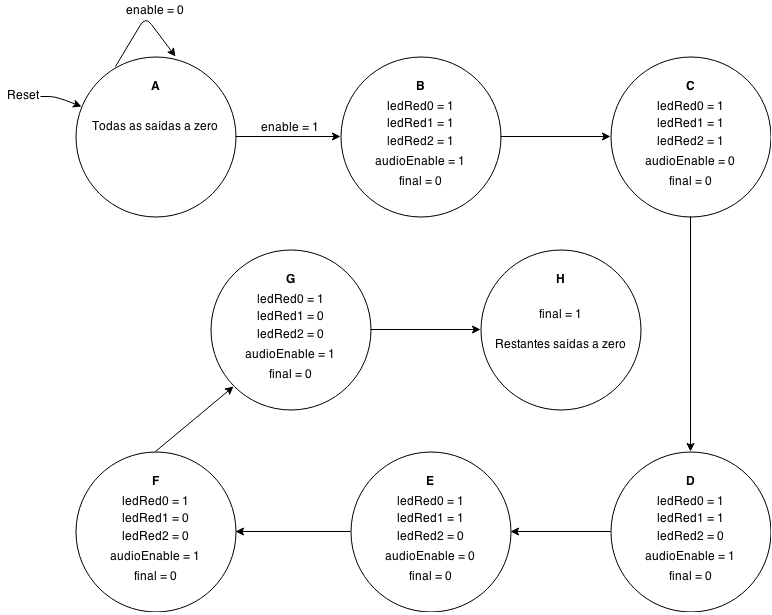
\includegraphics[scale=0.30]{Images/LEDCounterFSMDiagram}}
\caption{Arquitetura do \textit{LEDCounterFSM}.}
\label{figledcounterfsm}
\end{figure}

\subsection{\textit{TimerAux FSM}}

De seguida, assim que a máquina de estados anterior envie um sinal à \textit{Main FSM} de que terminou a sua ação (através do sinal \texttt{final}), a máquina principal envia um outro sinal (\texttt{newTime}) à \textit{TimerAux FSM}, para que se comece a contar o tempo até o LED indicador se acender.

Esta máquina, para além de receber um sinal para iniciar a contagem, consoante as entradas \texttt{defineRemote} e \texttt{defineSW}, que define se o tempo a contar é o selecionado no comando de infravermelhos ou 5 segundos, respetivamente, ou, por outro lado, se é um número aleatório recebido do bloco \texttt{random\_number\_generator} (valor este que é validado, pois apenas são aceites números entre 5 e 60 segundos).

Assim que a contagem chega a zero, a máquina envia um sinal a dizer que o tempo expirou e que já não está ativa (este último sinal permite que os sinais relativamente ao comando de infravermelhos sejam atualizados).

O diagrama da \textit{LEDCounter FSM} pode ser observado na \autoref{figtimerfsm}.

%figura 6%
\begin{figure}[h]
\centerline{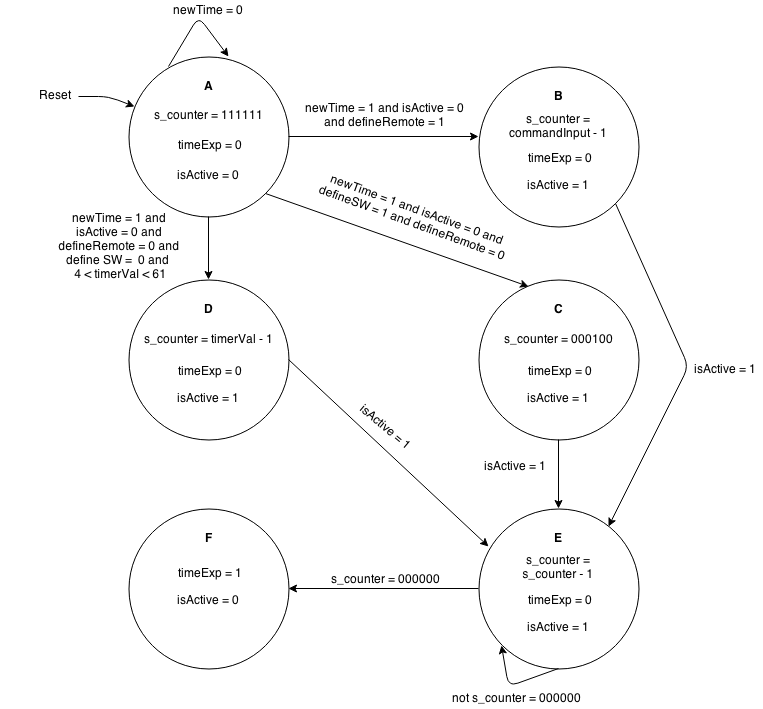
\includegraphics[scale=0.33]{Images/TimerAuxFSMDiagram}}
\caption{Diagrama de estados da \textit{Timer Aux FSM}.}
\label{figtimerfsm}
\end{figure}

Por fim, assim que a máquina de estados principal recebe o sinal \texttt{timeExp} ativo, acende o LED verde (indicador) e ativa o contador do tempo de reação (\textit{ReactionTimeCounter}), que funciona a uma frequência de 10000 Hz (também esta frequência foi gerada por um bloco \textit{FreqDivider}), isto é, irá apresentar o resultado até às décimas de milésimas. Ao mesmo tempo, também é ativado o bloco \texit{HexDisplay}, que interpreta o sinal vindo do contador e vai imprimindo nos ecrãs hexadecimais o tempo a percorrer.

Quando o utilizador carrega no botão de jogo, o contador pára e é impresso nos ecrãs o seu tempo de reação. No entanto, se carregar depois do sinal de partida, mas antes de o LED verde se acender, é impresso nos ecrãs hexadecimais uma mensagem de erro.

\section{Validação}

Apesar dos diversos blocos construídos, como alguns eram apenas de lógica simples (tais como o \textit{ReactionTimeCounter}, um simples contador com \texttt{enable}, e o \textit{HexDisplay}, que apenas converte um número binário de 24 dígitos para um formato de ecrã hexadecimal), decidiu-se apenas para validação das máquinas de estados, isto é, apenas foram desenvolvidas TestBenches para os blocos \textit{Main FSM}, \textit{TimerAux FSM} e \textit{LEDCounter FSM}.

\subsection{\textit{Main FSM}}
A construção da TestBench da máquina de estados principal (\textit{Main FSM}), seguiu dois caminhos: um em que não eram cometidos quaisquer erros e outro onde era cometido um erro, isto é, considerava-se que o botão de jogar estava ativo antes de o LED indicador se acender, o que iria provocar um erro.

Segue-se o gráfico resultante:

%figura 7%
\begin{figure}[h]
\centerline{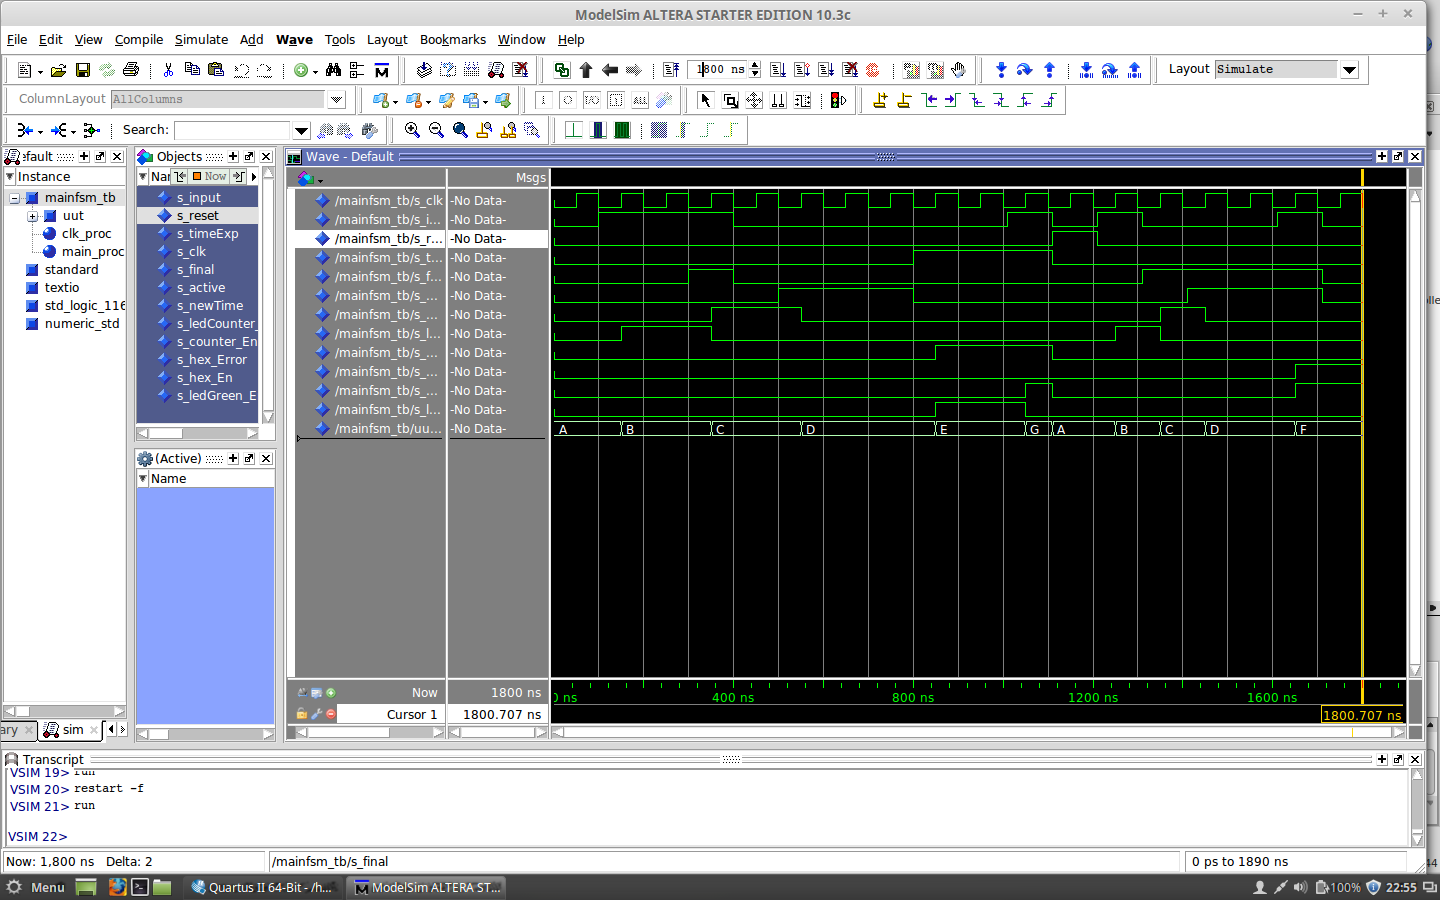
\includegraphics[scale=0.33]{Images/MainFSMTB}}
\caption{Gráfico da TestBench da \textit{Main FSM}.}
\label{figmainfsmtb}
\end{figure}

\subsection{\textit{TimerAux FSM}}

O desenvolvimento da TestBench deste bloco exigiu a sua separação em 3 situações: quando o tempo de reação é escolhido diretamente do comando de infravermelhos, quando é parametrizado para 5 segundos pelo \texttt{SW(0)} ou então sendo um valor aleatório entre 5 e 60.

A primeira situação foi do valor aleatório. Como estava ligado à entrada \texttt{timerVal} a saída do bloco \texttt{random\_number\_generator}, seria gerado um número aleatório a uma frequência de 50 MHz, e enquanto esse valor não fosse aceite (não estivesse no intervalo 5 a 60), a máquina não vai começar a subtrair o valor. Logo, neste teste, primeiro é fornecido um valor não válido e só depois um valido.

De seguida, é feito um \textit{reset} à máquina para ser testada com o tempo escolhido no comando de infravermelhos. Para o teste, foi fornecido o valor 7 (está no intervalo entre 1 e 9).

Por último, é testada a função de parametrizar através de um \textit{switch} da \ac{fpga}.

Segue-se o gráfico resultante:

%figura 7%
\begin{figure}[h]
\centerline{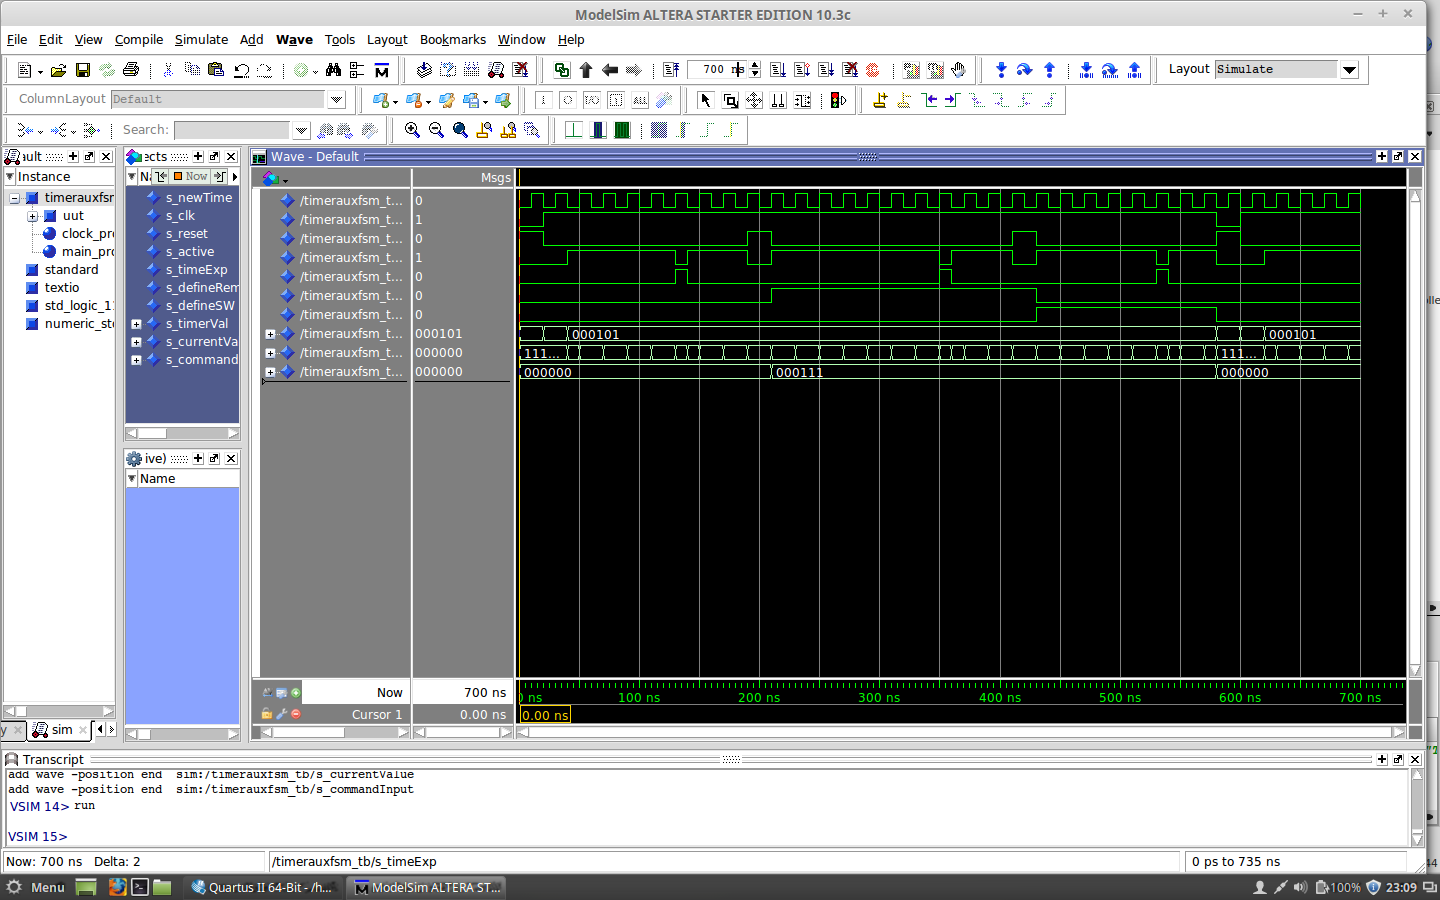
\includegraphics[scale=0.33]{Images/TimerAuxFSMTB}}
\caption{Gráfico da TestBench da \textit{TimerAux FSM}.}
\label{figtimerfsmtb}
\end{figure}

\subsection{\textit{LEDCounter FSM}}


\section{Manual de Instruções}
Para medir o seu tempo de reação, deve seguir os seguintes passos:
\begin{itemize}
\item Certificar-se que a \ac{fpga} está corretamente ligada e programada;
\item Pressionar o botão \texttt{KEY(0)} (Play no comando de infravermelhos), para iniciar o jogo;
\item Pode desligar o som da placa ativando o \texttt{SW(1)} ou clicando no botão de Mute do comando de infravermelhos;
\item Pode também parametrizar o tempo que demora a acender o LED verde, acionando o \texttt{SW(1)} (5 segundos de espera), ou escolhendo um valor entre 1 e 9 no comando de infravermelhos e pressionando a tecla QUALQUERCOISA;
\item Aguardar que os três LED vermelhos se apaguem;
\item Clicar no botão \texttt{KEY(0)} (ou Play no comando de infravermelhos), logo depois de o LED verde se acender;
\item Será impresso no ecrã hexadecimal o seu tempo de reação;
\item Para reiniciar o jogo, basta pressionar \texttt{KEY(1)} (ou Return no comando de infravermelhos) e repetir todos os passos acima descritos.
\end{itemize}


\chapter{Conclusões}
\label{chap.conclusao}
Em suma, depois de estabelecida a arquitetura do sistema, os vários diagramas de estados e a divisão de tarefas, é possível passar à prática e programar o circuito.


%%%%%%%%%%%%%%%%%%%%%%%%%%%%%%%%%
\chapter*{Acrónimos}
\begin{acronym}
\acro{ua}[UA]{Universidade de Aveiro}
\acro{miect}[MIECT]{Mestrado Integrado em Engenharia de Computadores e Telemática}
\acro{fpga}[FPGA]{Field-Programmable Gate Array}
\acro{vhdl}[VHDL]{Very high speed integrated circuit Hardware Description Language}

\end{acronym}


%%%%%%%%%%%%%%%%%%%%%%%%%%%%%%%%%

\end{document}
